\thispagestyle{empty}
\begin{center}
%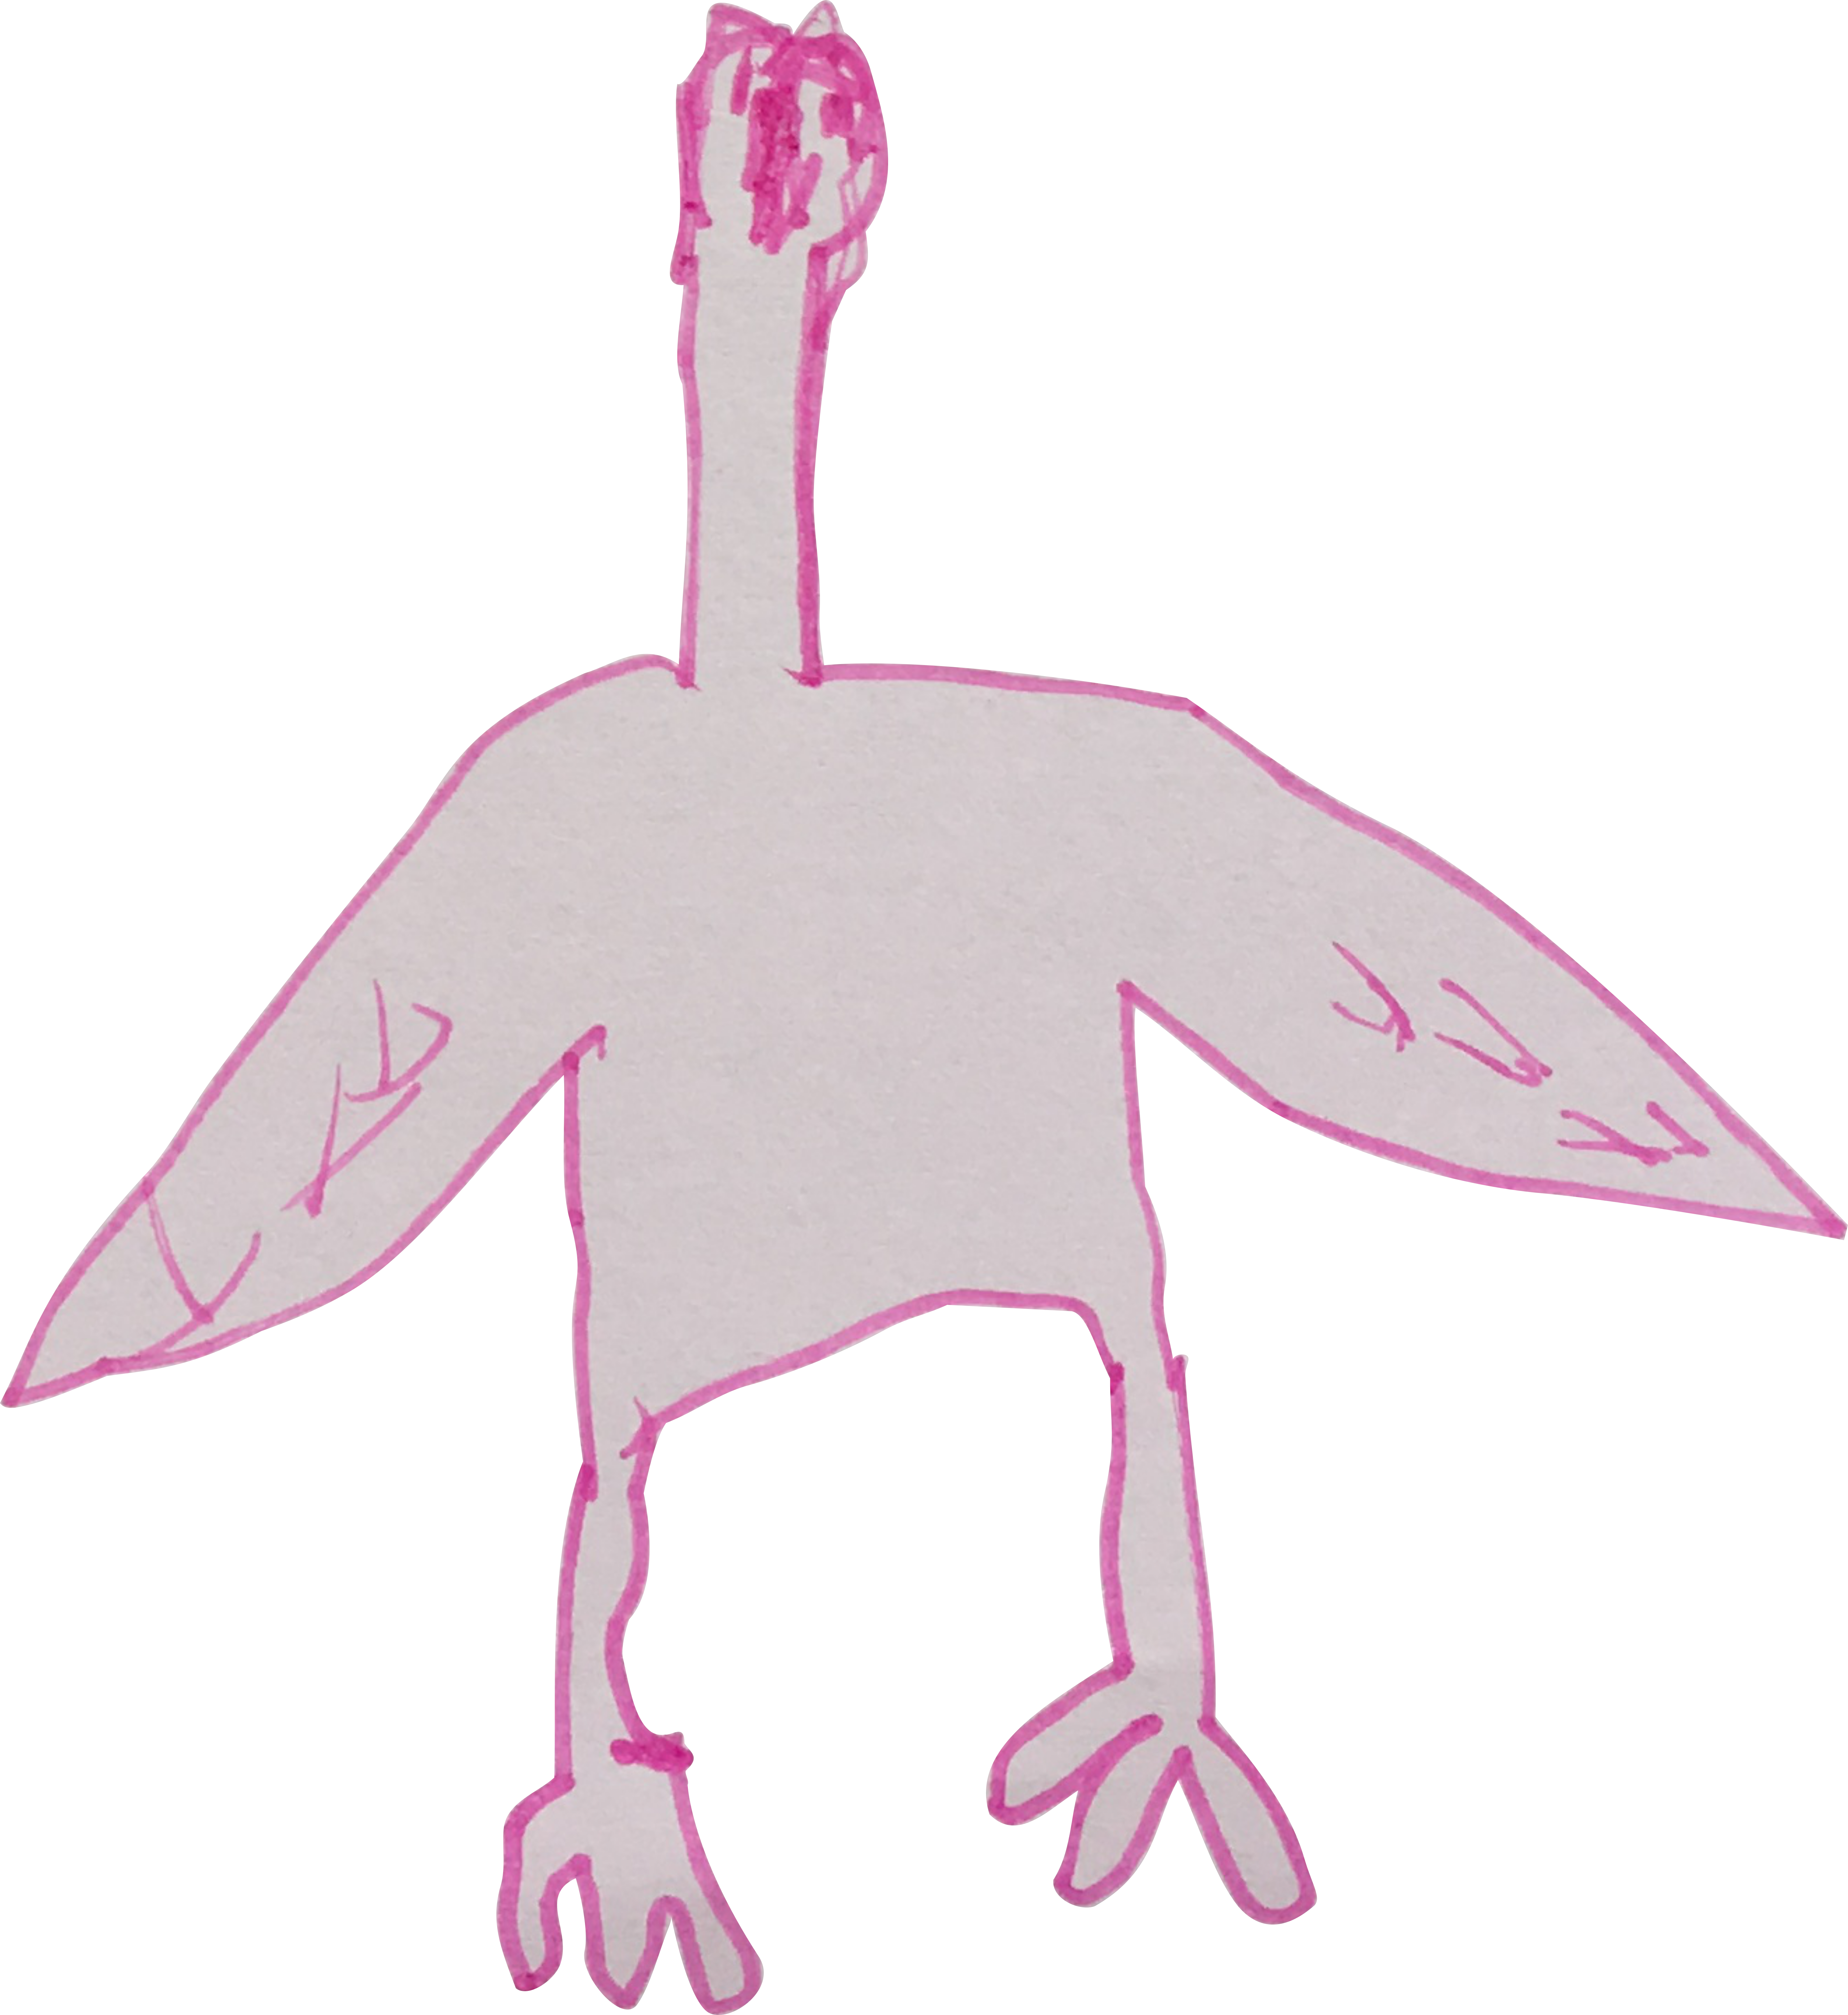
\includegraphics[height=.7\textheight]{./bilder/huhn2.png}
\end{center}
\vskip 2cm
{\Huge\color{farbe}\hfill{\tt{Leo}}}
\addcontentsline{toc}{chapter}{Leo}
\newpage
%%%%%%%%%%%%%%%%%%%%%%%%%%%%%%%%%%%%%%%%%%%%%%%%%%%%%%%%%%%%%%%%%%%%%%%%%%%%%%%
\lettrine[lines=2, lhang=.2, loversize=.25, lraise=0.05, findent=0.1em,
nindent=0em]{{\textooquote}A}{}lle Kinder anziehen bitte! Wir gehen jetzt raus und spielen Schatzsuche.\textcoquote Aysel Ocak aus dem Kindergarten hat Geburtstag. Elin ist auch eingeladen, aber sie kennt hier niemanden. Alles nur Cousins und Cousinen von Aysel, die sich auf Kurdisch unterhalten, und das kann Elin nicht so gut. Papa will zwar immer mit ihr üben, aber sie kann sich einfach kein Wort merken. Frau Ocak spricht nur wegen ihr Deutsch mit allen.

Und jetzt Schatzsuche. Alle rufen wild durcheinander und Frau Ocak kommt gar nicht hinterher, alle Schuhe zu binden. Eilen ist die letzte, die dran kommt. Da hat ihr Papa wohl doch Recht gehabt, hätte sie mal lieber Kurdisch mit ihm geübt.

Als sie endlich auch fertig ist, sind die anderen Kinder schon mit dem Lift die sieben Stockwerke nach unten gefahren und zum kleinen Wäldchen gelaufen. Frau Ocak versucht zwar zu rufen, die Kinder sollen mal nach Hinweisen suchen, aber der Schatz ist bereits entdeckt. In einem hohlen Baum, da hätte Eilen auch als erstes nachgesehen. 

Wenn man kein Wort versteht, ist man schnell alleine, das merkt Eilen jetzt. Sie beschliesst, selbst noch nach Hinweisen zu suchen. Im Wäldchen kennt sie sich gut aus, hier spielt sie selber auch oft. 

Sie findet einen grossen Luftballon mit einem Pfeil darauf. Der hat sich allerdings so in einem Baum verfangen, dass er sich durch den Wind in alle Richtungen dreht. Eilen wartet, bis der Pfeil auch einmal in die Richtung zeigt, in der sie am liebsten weiter suchen will und geht dann los.

Plötzlich kracht und zischt es ganz gewaltig direkt vor ihr. Äste brechen , die Vögel fliegen aufgeregt davon. Eilen rennt auch los, bleibt aber schon nach dem ersten Sprung mit den Haaren in einem Gebüsch hängen. 

\enquote{Au, au, au, au}

Als sie versucht sich zu befreien, hört sie etwas sehr Merkwürdiges. Ist das jetzt ein Tier gewesen oder nicht? Egal, es klingt wie ein Hilfeschrei. Endlich die Haare bfreien und dann los.  Und Eilen sieht: nichts. Nur der Wald genau so wie er immer ist, nirgends scheint etwas anders zu sein als sonst. Komisch, staunt Eilen. Aber dann hört sie es wieder. Aus dem Schrei ist ein Wimmern geworden, viel leiser als vorhin, und  ganz in ihrer Nähe. Sie sieht sich um und sieht einen Hund. Aber keinen echten, sondern einen aus Plüsch. 

Ob der das wohl gewesen ist? Nein, das ist ganz und gar unmöglich. Eilen hebt den Hund hoch und \dots

\enquote{Da bist du ja!} Frau Ocak kämpft sich durch das Dickicht des Wäldchens. \enquote{Dein Eltern sind schon da und warten auf Dich!}

\enquote{Aber da war etwas, haben sie das nicht gehört?} Aber Frau Ocak hat keinen Sinn für Kindergeschichten und ist schon wieder auf dem Weg zurück. Eilen wirft einen letzten Blick zurück und trottet hinterher.

Im Auto auf der Fahrt nach Hause fragt ihre Mama, was das für ein furchtbar schmutziges Ding sei, dass sie da habe und das ihr das nicht in die Wohnung käme. Erst da wird Eilen bewusst, dass sie den Plüschhund immer noch hat. 

Ohne zu überlegen antwortet Eilen, dass dies Leo sei, der wohne jetzt bei ihr. Natürlich ist Mama dagegen. Sie sagt etwas von\dots, aber das hört Eilen schon alles gar nicht mehr. Denn der Hund hat gezwinkert. Der Plüschhund hat gezwinkert. Und sie dabei angesehen. Eilen hatte mal so ein Puppe, die hat die Augen geschlossen, wenn man sie hingelegt hat. Und Leo kann das also auch.

Der Kompromis, den Papa gerade mit Mama ausgehandelt hat ist, dass Papa den Hund als erstes in die Waschmaschine stecken wird. Wenn er das überlebt und nicht ganz zerfällt, darf er bleiben.

Am Abend kommt Papa mit Leo aus dem Keller. Leo scheint ein Dackel zu sein, aber ganz sicher ist sich niemand. Jedenfalls muss Mama zugeben, dass Leo wirklich sauber zu sein scheint und erteilt die Wohnerlaubnis. Vorläufig.

Gutenachtkuss eins kommt heute von Papa, Nummer zwei von Mama. Die Tür muss einen Spalt offen bleiben, wie immer, Licht aus.

\enquote{Leo darf neben dem Bett Wache halten.} sagt Mama im Rausgehen. Damit will sie sagen, dass er nicht mit ins Bett darf, Waschmaschine hin oder her. Sobald es ruhig ist und auch Mama die Treppe runter in Wohnzimmer gegangen ist, hört Eilen leise Tritte in ihrem Zimmer, sie hält die Luft an, dann geht die Tür zu und noch ehe sie laut schreien kann, geht das Licht an. 

Leo ist gegen den Schalter gesprungen. Leo ist gegen den Schalter gesprungen? 

\enquote{Ich bin jetzt so und so viele Lichtjahre durchs Weltall geflogen. Durch die halbe Galaxie nehme ich an. Aber das war alles nichts im Vergleich zu einer Stunde in eurer Waschmaschine. Begrüsst ihr Besucher von anderen Planeten immer so? Himmel, ich bin so durcheinander wie damals, als ich als vierunvierzig jähriges Kind auf Golgator\,7 im Freizeitpark mit dem Achterraumschiff geflogen bin. Das hier war sogar schlimmer, aber irgendwie auch\dots gross-ar-tig! Ich heisse übrigens Leo}

Eilen war so verwirrt, dass ihr als Antwort nichts anderes einfel als:

\enquote{Ich weiss, dass du Leo bist.}

\enquote{Euer kleiner Planet gefällt mir gut! Ein bisschen blau, aber ganz nett. Auf Frululu, wo ich her komme, regnet es immer. Allerdings je nach Jahreszeit in anderen Farben, wir haben übrigens 27. Ein Tag dauert aber nur drei Erdenstunden und die Nacht auch nochmals so viel. Ich schlafe daher öfter als du, aber nicht so lange, Gute Nacht.}

Und damit schlief Leo ein, schneller als Papa. Er sah jetzt wieder aus, wie ein ganz normaler Plüschhund. Eilen war sprachlos, sie wusste gar nicht, was sie denken oder machen sollte. Und schlief dann auch ein.


Am nächsten Morgen, dauerte der Moment, bei dem man nicht so sicher ist, ob man noch träumt oder schon wach ist, besonders lange bei Eilen. War das gestern wirklich alles passiert?

\enquote{Guten Morgen!} Leo war schon wach und sass auf ihrem Schreibtisch. Vor sich eine CD, die er als Spiegel zu benutzen schien. Und den Schminkkoffer von Eilen. Seine Schnauze hatte er bereits rot gefärbt, jetzt 








\vfill
